\section{实验结果样例}
本章用于测试宽表格、多行表格、多子图和图表交叉引用。实验内容参考源论文中的桥接分数分析与压缩结果，但数值仅作为模板排版样例。

\subsection{评测任务与指标}
评测任务分为多模态和纯文本两类，如\tabref{chart:tasks}所示。多模态任务可使用LMMs-Eval进行评测\cite{zhang2024lmmseval}，其中InfoVQA、MMMU和OCRBench分别覆盖信息图问答、多学科视觉理解和OCR能力\cite{mathew2022infographicvqa,yue2024mmmu,liu2024ocrbench}。

\begin{table}[!ht]
    \centering
    \caption{评测任务配置}
    \label{chart:tasks}
    \begin{tabular}{llll}
    \toprule
        类别 & 任务 & 指标 & 评测内容 \\ \midrule
        \multirow{3}{*}{多模态} & InfoVQA (val\_lite) & ANLS & 信息图理解与问答 \\
        & MMMU (val) & Acc & 多学科多模态理解 \\
        & OCRBench & Acc & 光学字符识别 \\ \midrule
        \multirow{3}{*}{文本} & ARC-Easy & Acc & 科学常识推理 \\
        & WinoGrande & Acc & 常识推理 \\
        & PIQA & Acc & 物理直觉推理 \\
    \bottomrule
    \end{tabular}
\end{table}

核心评估指标为保留率，定义为压缩后模型在特定任务上的分数与基准模型分数的比值，如\eqnref{eq:retention}所示。
\begin{equation}
    \label{eq:retention}
    \text{Retention}(\%) = \frac{\text{Score}_{\text{compressed}}}{\text{Score}_{\text{base}}} \times 100\%
\end{equation}

\subsection{宽表格测试}
\tabref{chart:50pct}用于检查9列宽表格、分组表头、\verb|\cmidrule|、粗体数值和英文缩写在DOCX中的换行效果。

\begin{table}[!ht]
    \centering
    \caption{DeepSeek-VL2-Small 50\%保留率（64$\to$32专家）保留率(\%)对比}
    \label{chart:50pct}
    \setlength{\tabcolsep}{4pt}
    \fitwidetable{%
    \begin{tabular}{lcccccccc}
    \toprule
        \multirow{2}{*}{方法} & \multicolumn{4}{c}{多模态任务} & \multicolumn{4}{c}{文本任务} \\
        \cmidrule(lr){2-5} \cmidrule(lr){6-9}
        & InfoVQA & MMMU & OCR & 平均 & ARC-E & WinoG & PIQA & 平均 \\ \midrule
        MergeMoE & 35.2 & 51.9 & 15.5 & 34.2 & 44.9 & 75.4 & 76.3 & 65.5 \\
        HC-SMoE & 80.8 & 61.4 & 77.6 & 73.2 & 71.7 & 81.9 & 84.7 & 79.4 \\
        HC-SMoE+桥接 & 77.3 & 67.6 & 81.9 & 75.6 & 70.8 & 85.8 & \textbf{90.0} & 82.2 \\
        MC-SMoE & 0.0 & 58.0 & 2.2 & 20.1 & 43.1 & 75.3 & 75.4 & 64.6 \\
        MC-SMoE+桥接 & 69.7 & 60.9 & 59.9 & 63.5 & 50.4 & 76.6 & 77.5 & 68.2 \\
        REAP & 77.0 & 76.8 & 76.6 & 76.8 & 53.8 & 79.8 & 81.5 & 71.7 \\
        REAP+桥接 & \textbf{85.0} & \textbf{84.5} & \textbf{82.9} & \textbf{84.1} & \textbf{81.5} & \textbf{88.0} & 88.5 & \textbf{86.0} \\
    \bottomrule
    \end{tabular}%
    }
\end{table}

\subsection{图片测试}
\figref{fig:bridge_score_comparison}用于检查单张宽图的排版效果。该图展示了桥接分数对比，适合观察图片是否过窄、标题是否紧贴图片、编号是否按章重排。

\begin{figure}[!ht]
    \centering
    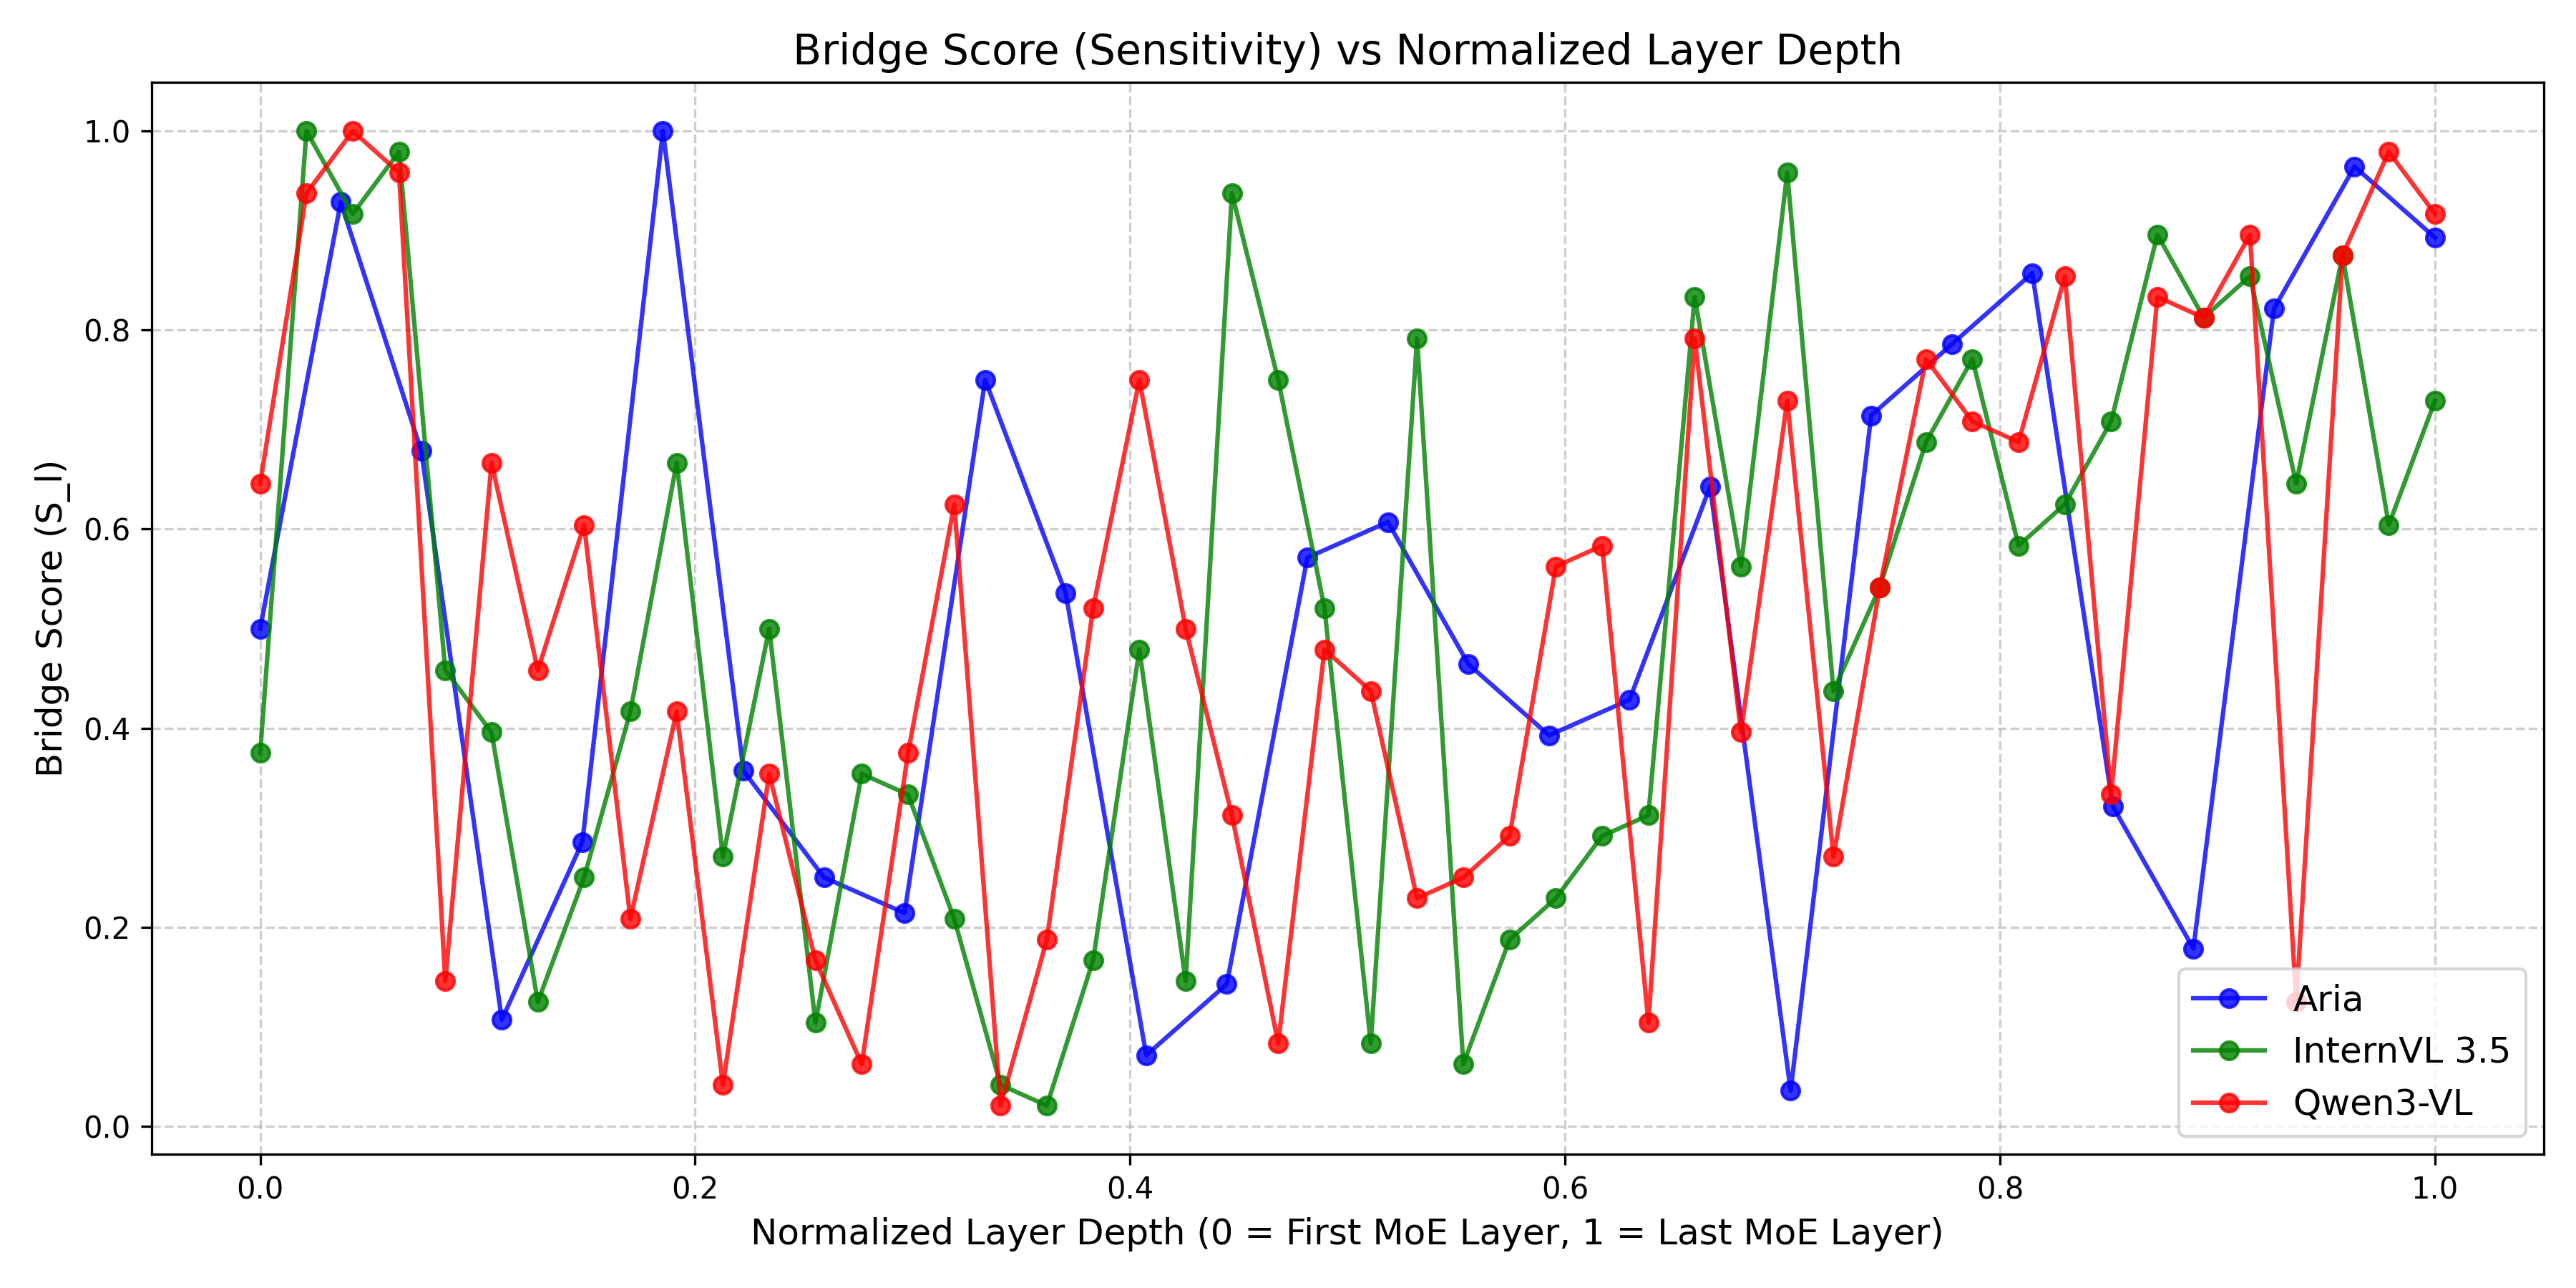
\includegraphics[width=0.88\textwidth]{images/bridge_score_comparison.png}
    \caption{不同模型中的桥接分数对比示意}
    \label{fig:bridge_score_comparison}
\end{figure}

除单张图外，\figref{fig:cross_model_heatmap_extra}提供三张子图组合，用于检查子图在Word中的行内布局和整体图题位置。Qwen3-VL、InternVL和Aria均为近期多模态模型或MoE多模态模型代表\cite{bai2025qwen3vl,wang2025internvl35,li2024aria}。

\begin{figure}[H]
    \centering
    \subfigure[Qwen3-VL]{
        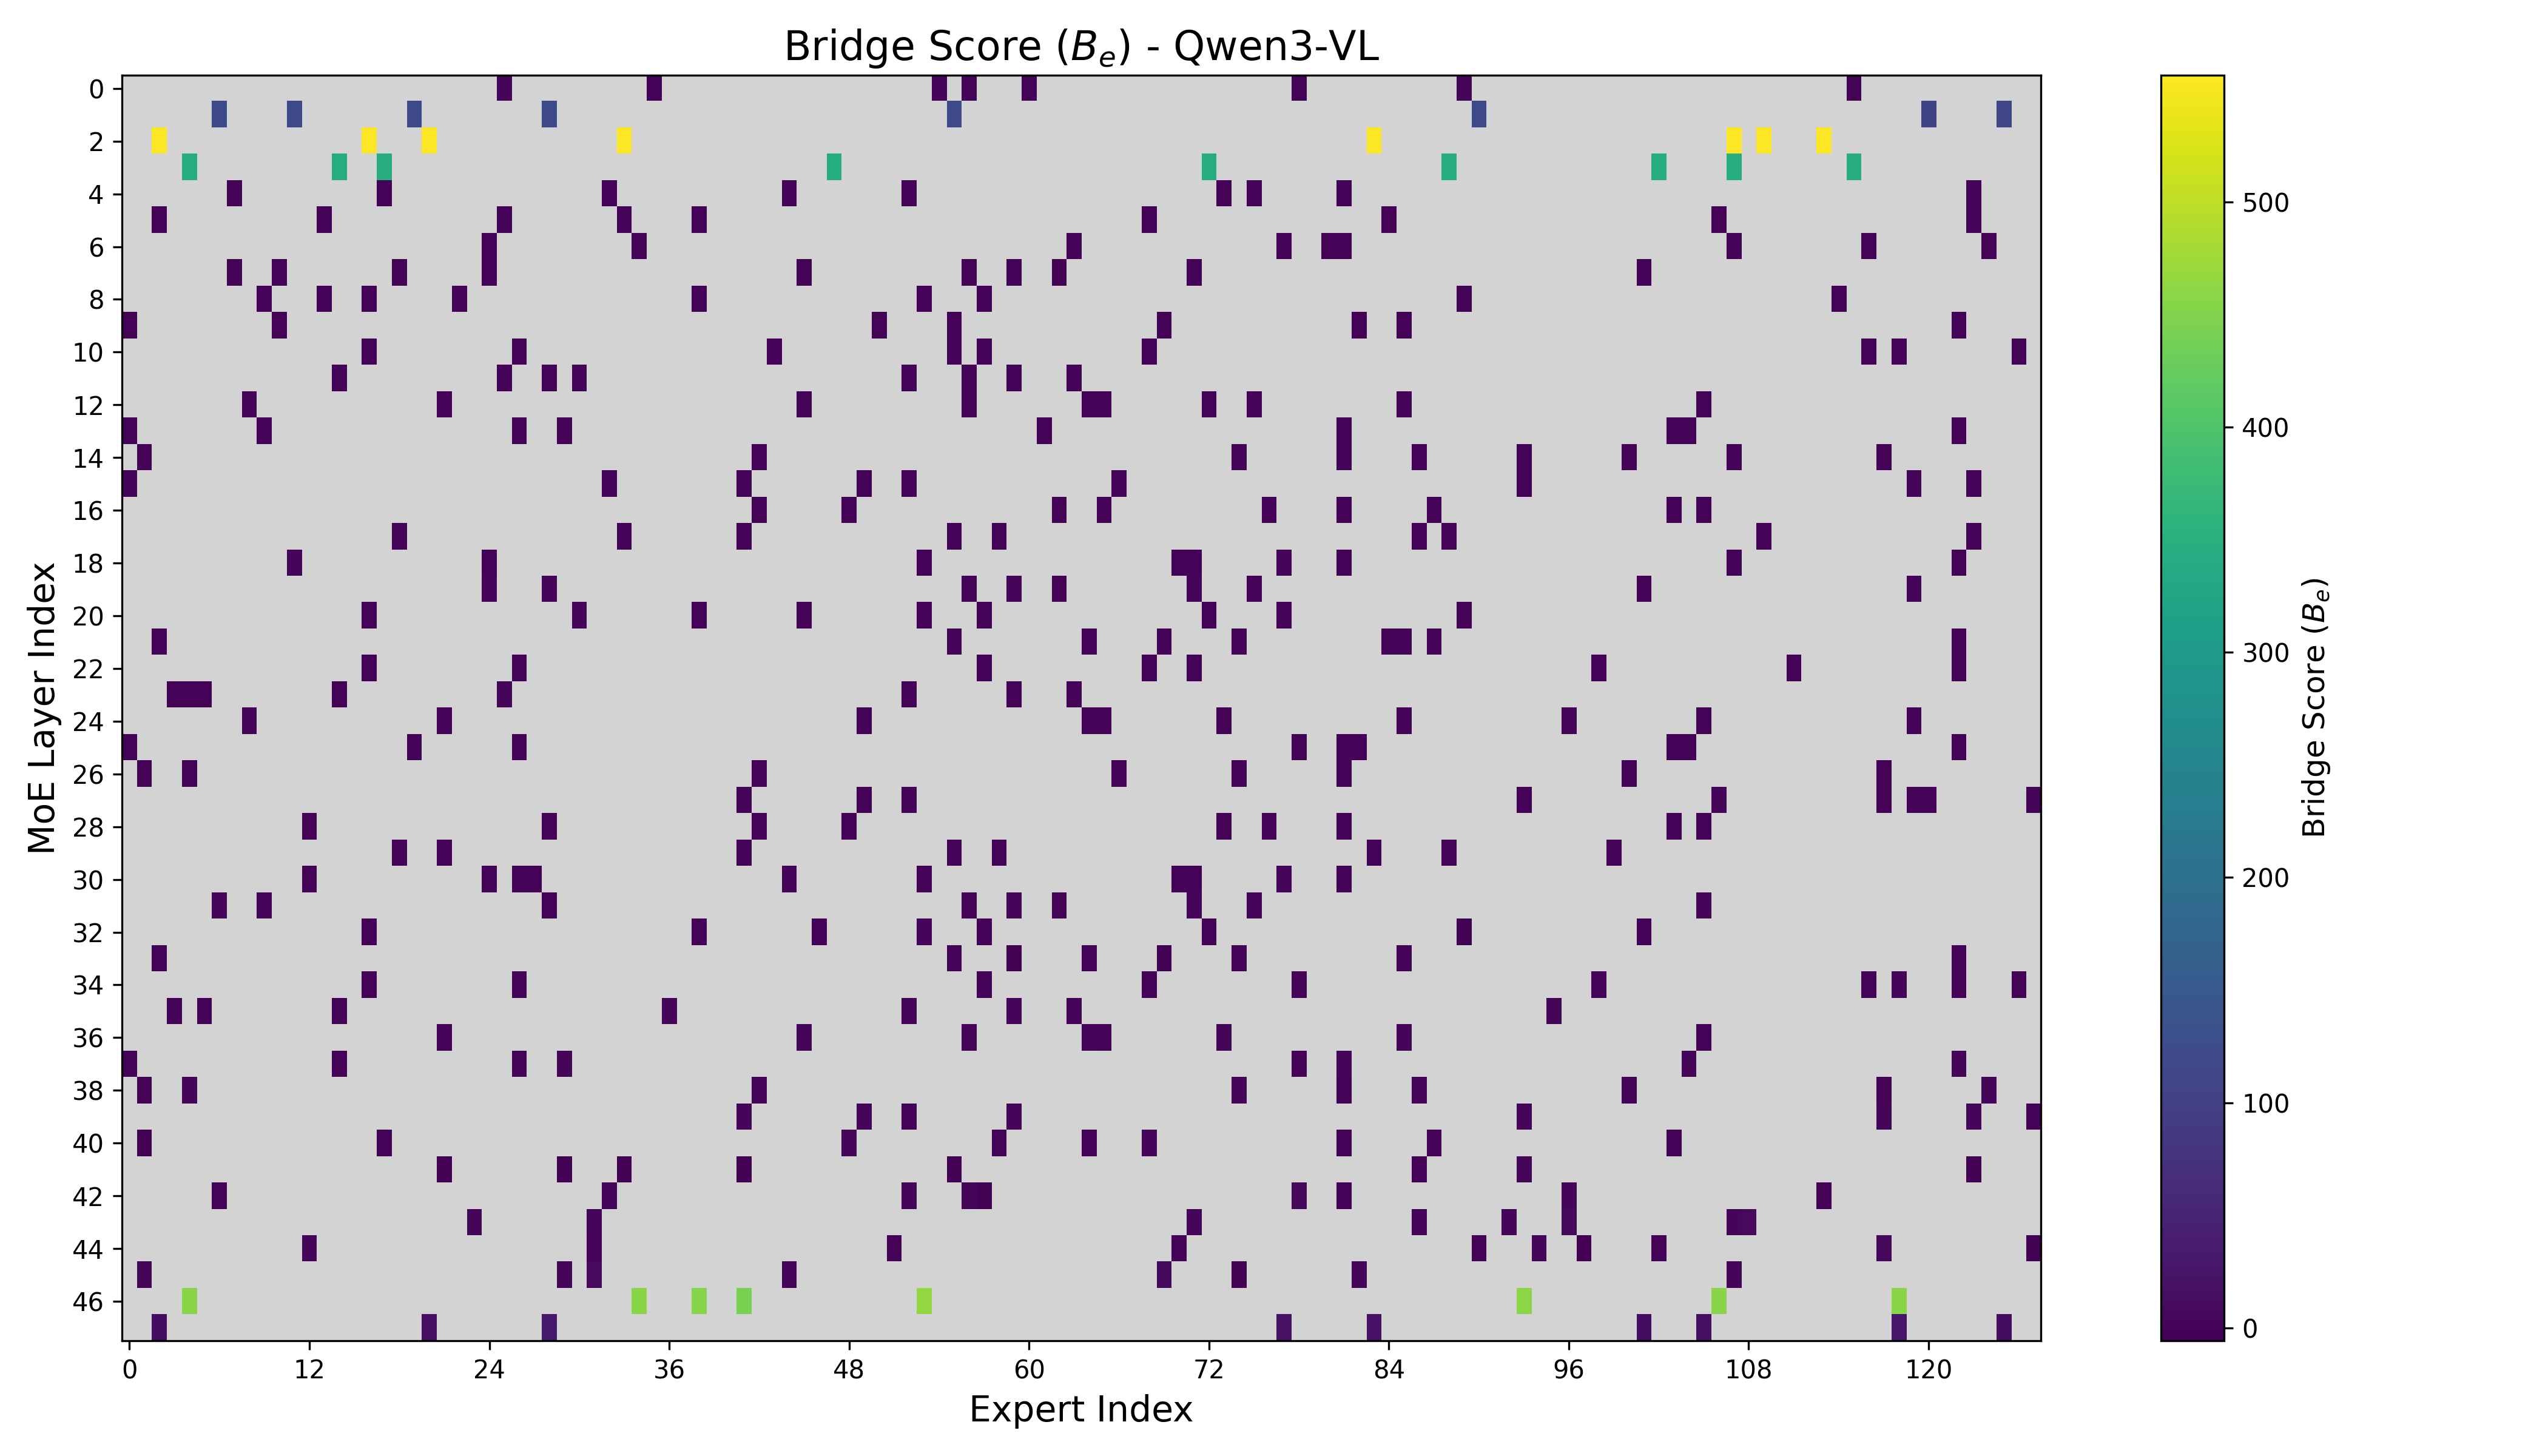
\includegraphics[width=0.48\textwidth]{images/bridge_heatmap_qwen3vl.png}
    }
    \subfigure[InternVL]{
        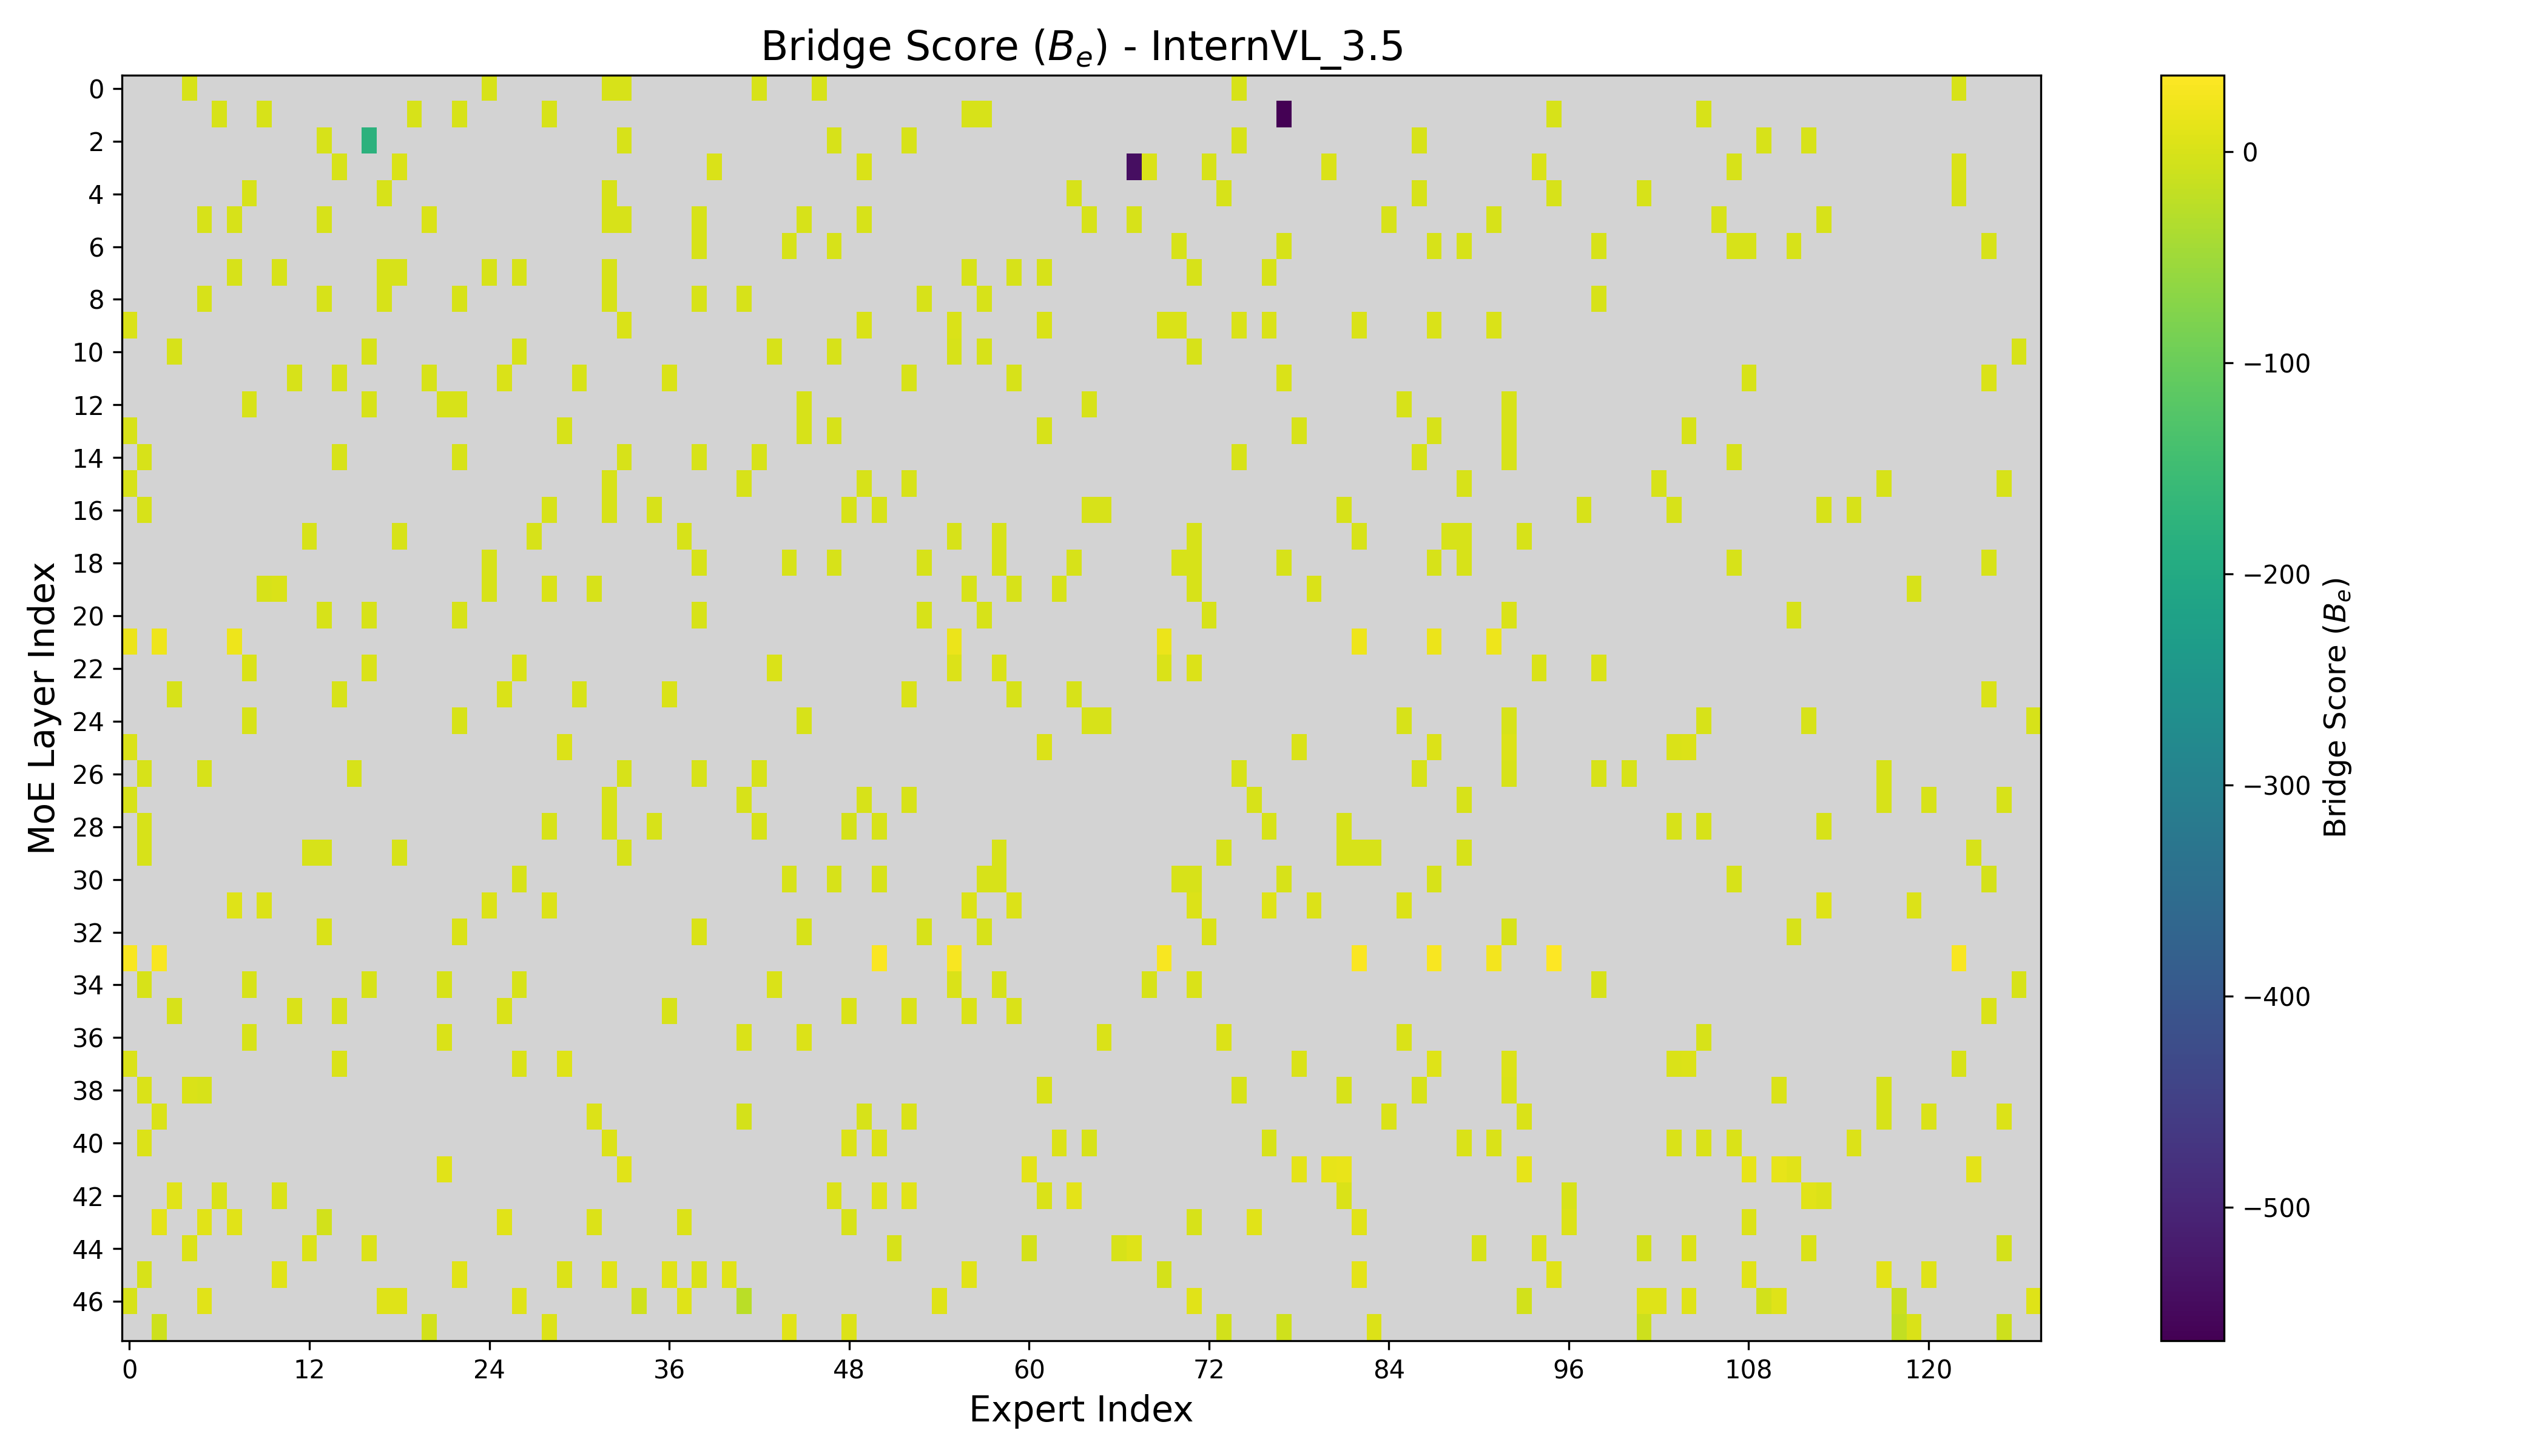
\includegraphics[width=0.48\textwidth]{images/bridge_heatmap_internvl.png}
    }

    \subfigure[Aria]{
        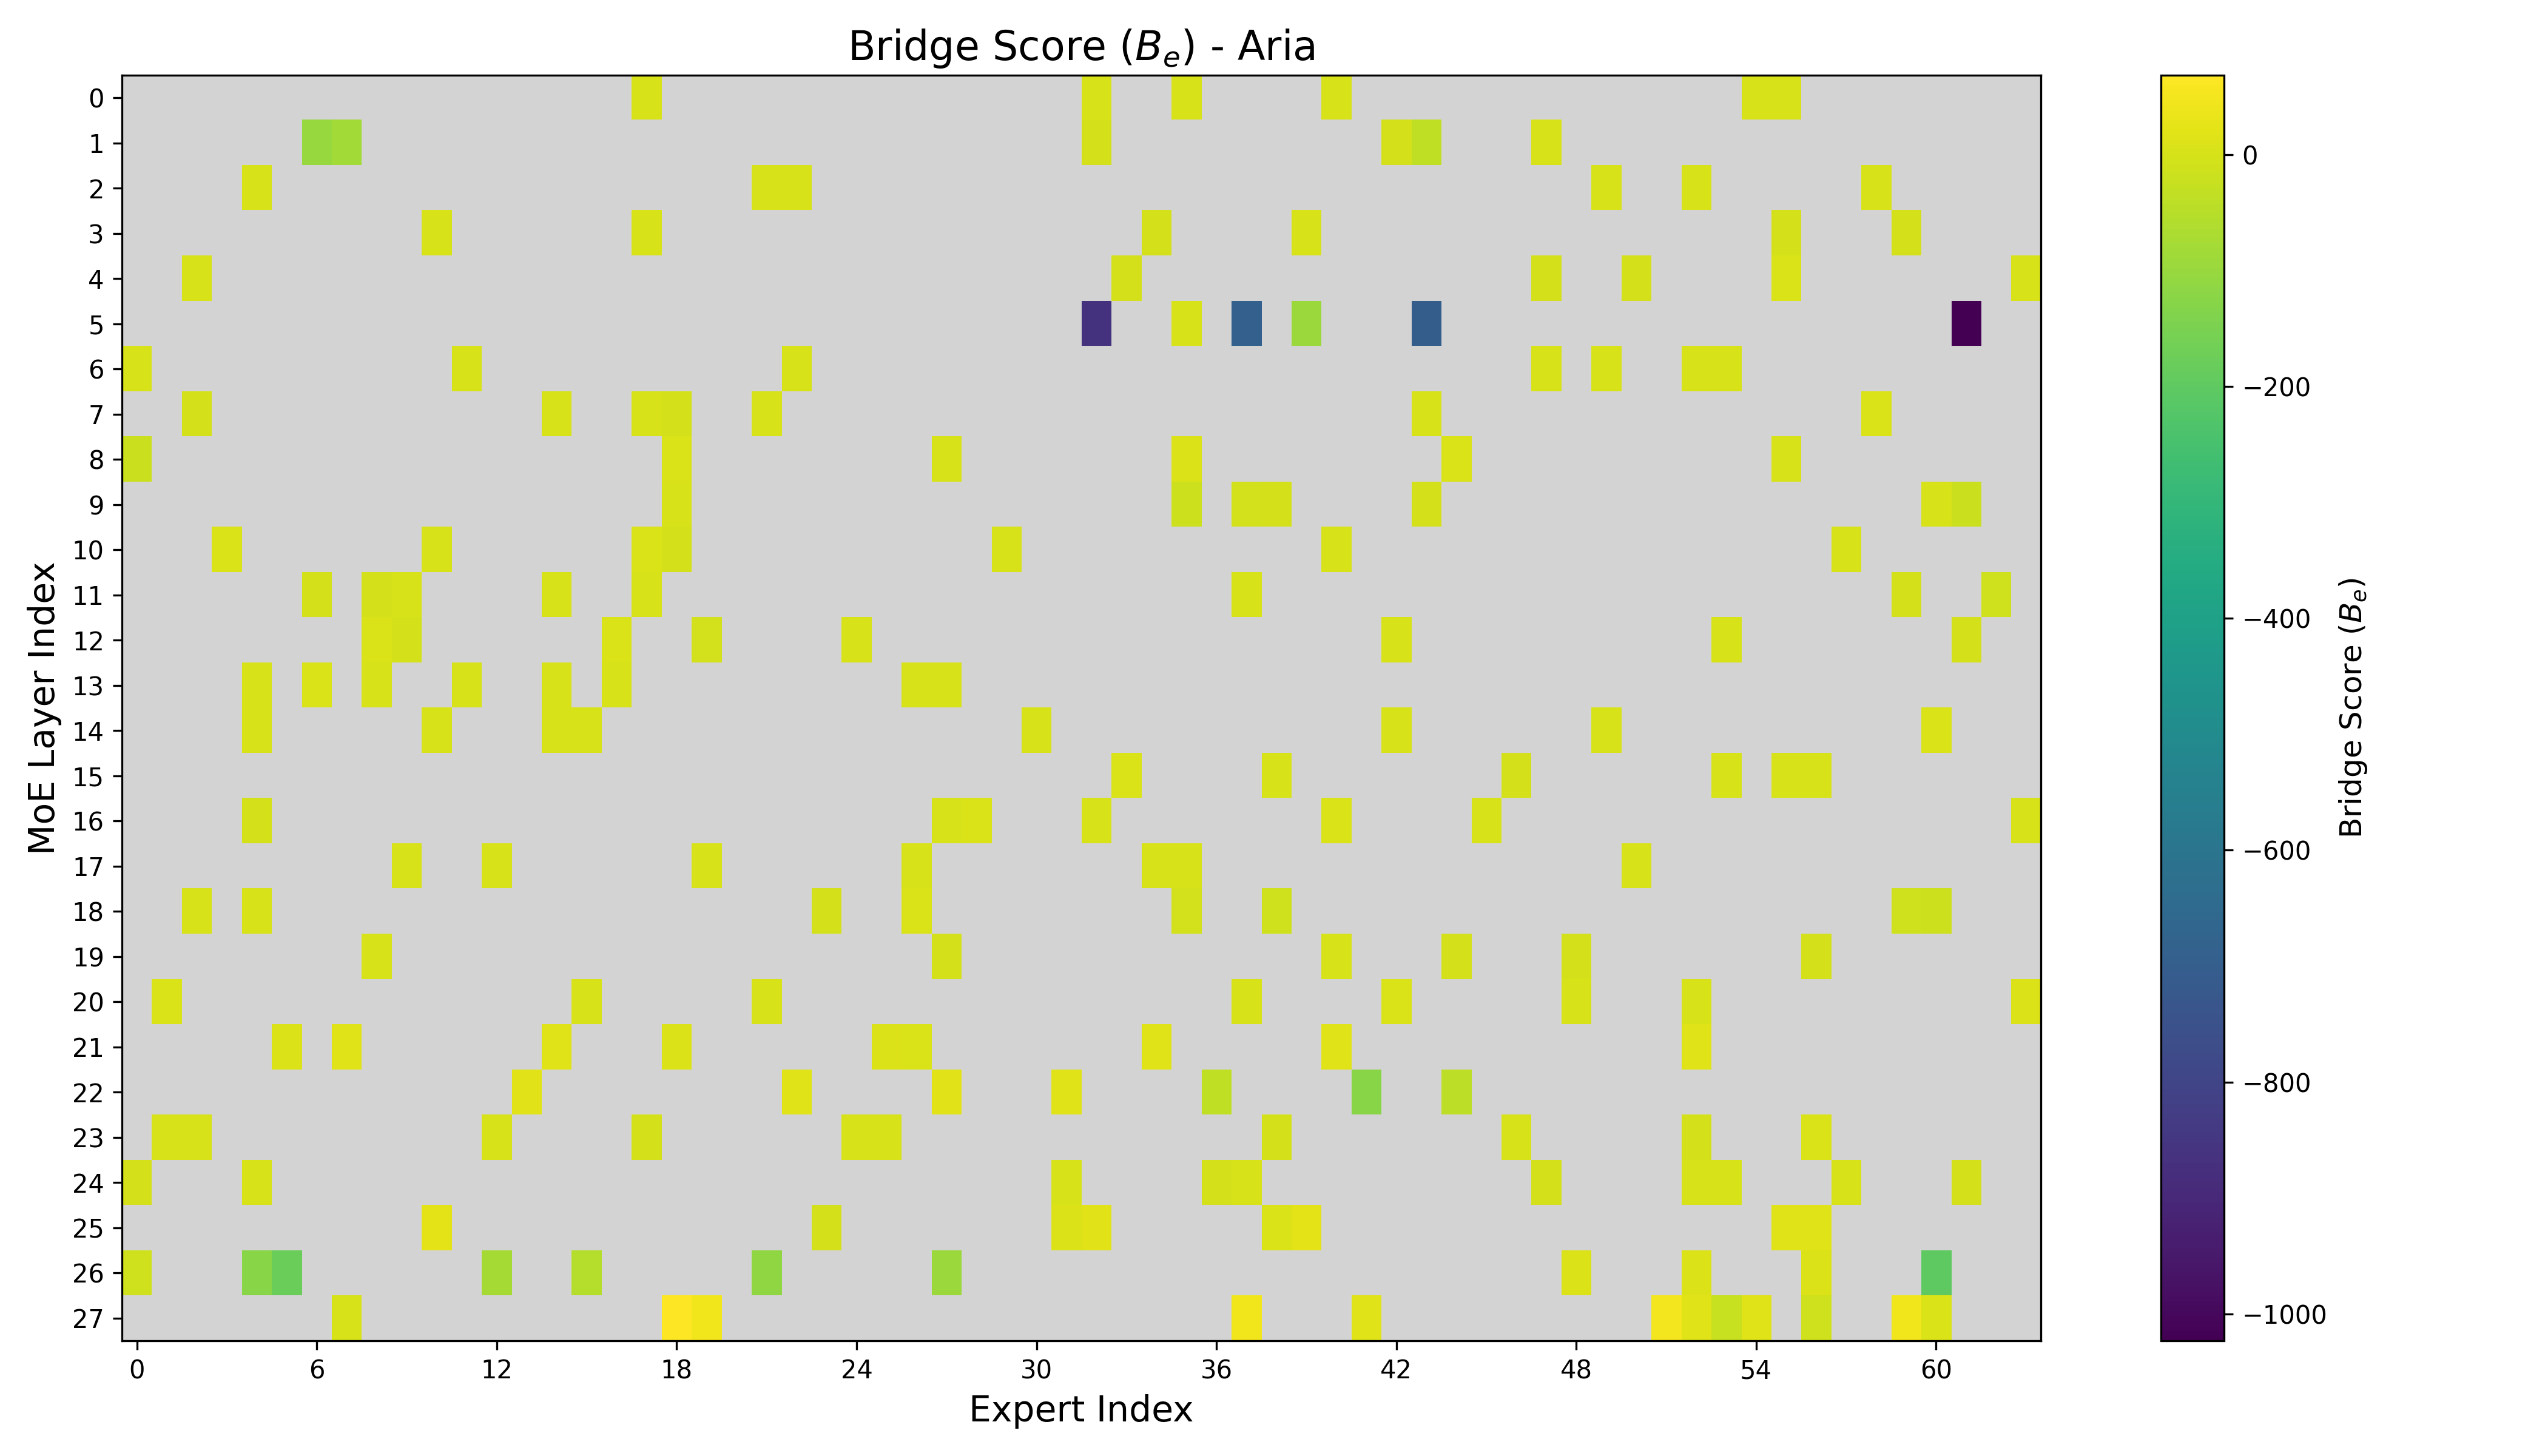
\includegraphics[width=0.62\textwidth]{images/bridge_heatmap_aria.png}
    }
    \caption{跨模型桥接分数热力图排版测试}
    \label{fig:cross_model_heatmap_extra}
\end{figure}

\subsection{本章小结}
本章提供了多行表、宽表、单图和多子图测试。转换后建议重点检查\tabref{chart:tasks}、\tabref{chart:50pct}、\figref{fig:bridge_score_comparison}和\figref{fig:cross_model_heatmap_extra}的显示效果。
